\documentclass[11pt]{article}

\usepackage[a4paper, margin=1in]{geometry}
\usepackage{graphicx}
\usepackage{booktabs}
\usepackage{amsmath, amssymb}
\usepackage[expansion=false]{microtype}
\usepackage{hyperref}
\usepackage{xcolor}
\usepackage{authblk}
\usepackage{natbib}
\usepackage{float}
\usepackage[font=small,labelfont=bf]{caption}
\usepackage{placeins}
\bibliographystyle{plainnat}

\hypersetup{
  colorlinks=true,
  linkcolor=black,
  citecolor=blue!50!black,
  urlcolor=blue!50!black,
}

\title{Comment on Olalde et al.\ 2023:\
       the omitted NorthMacedonia\_IA substrate in the 1-source qpAdm screen}

\author{\textit{Nikola Tsartsarov}}

\date{\today}

\begin{document}

\maketitle
\newcommand{\BestPublishedMinP}{0.0016}
\newcommand{\BestPublishedMinTarget}{Croatian}
\newcommand{\BestPublishedMaxP}{0.0401}
\newcommand{\BestPublishedMaxTarget}{Albanian}
\newcommand{\NorthmacMinP}{0.246}
\newcommand{\NorthmacMinTarget}{Romanian}
\newcommand{\NorthmacMaxP}{0.971}
\newcommand{\NorthmacMaxTarget}{Albanian}


\begin{abstract}
\noindent
\citet{Olalde2023} begin their present-day Balkan qpAdm analysis with a
1-source substrate screen reported in Data~S1 \S5 and Data~S2 Table~8. This
comment addresses one narrow methodological point in that screen. We restate it
on the exact public AADR Human Origins labels available in the dataset used in
this analysis: \texttt{Croatian}, \texttt{Serbian\_Serb},
\texttt{Romanian}, \texttt{Bulgarian}, \texttt{Albanian}, \texttt{Greek}, and
\texttt{Cypriot}. Under the documented setup, all six published local
substrate columns fail across this retained panel. We then add one plausible
omitted Iron Age Balkan candidate, \texttt{NorthMacedonia\_IA}, which was
publicly available before \citet{Olalde2023} and lies in the same broad
regional and chronological frame as several published substrates.

The result is straightforward. On this strict public-label panel, every
published substrate column remains rejected under \texttt{allsnps=TRUE},
whereas the added \texttt{NorthMacedonia\_IA} column passes all seven retained
rows, with p-values ranging from \NorthmacMinP{} to \NorthmacMaxP{}. It shows
that the published first-stage local-substrate screen was not exhaustive even at the simplest
1-source level. For a screening step used to constrain later model choice, one
relevant omitted candidate that reverses the pass/fail pattern is sufficient to
demonstrate that point.
\end{abstract}

\begin{figure}[H]
  \centering
  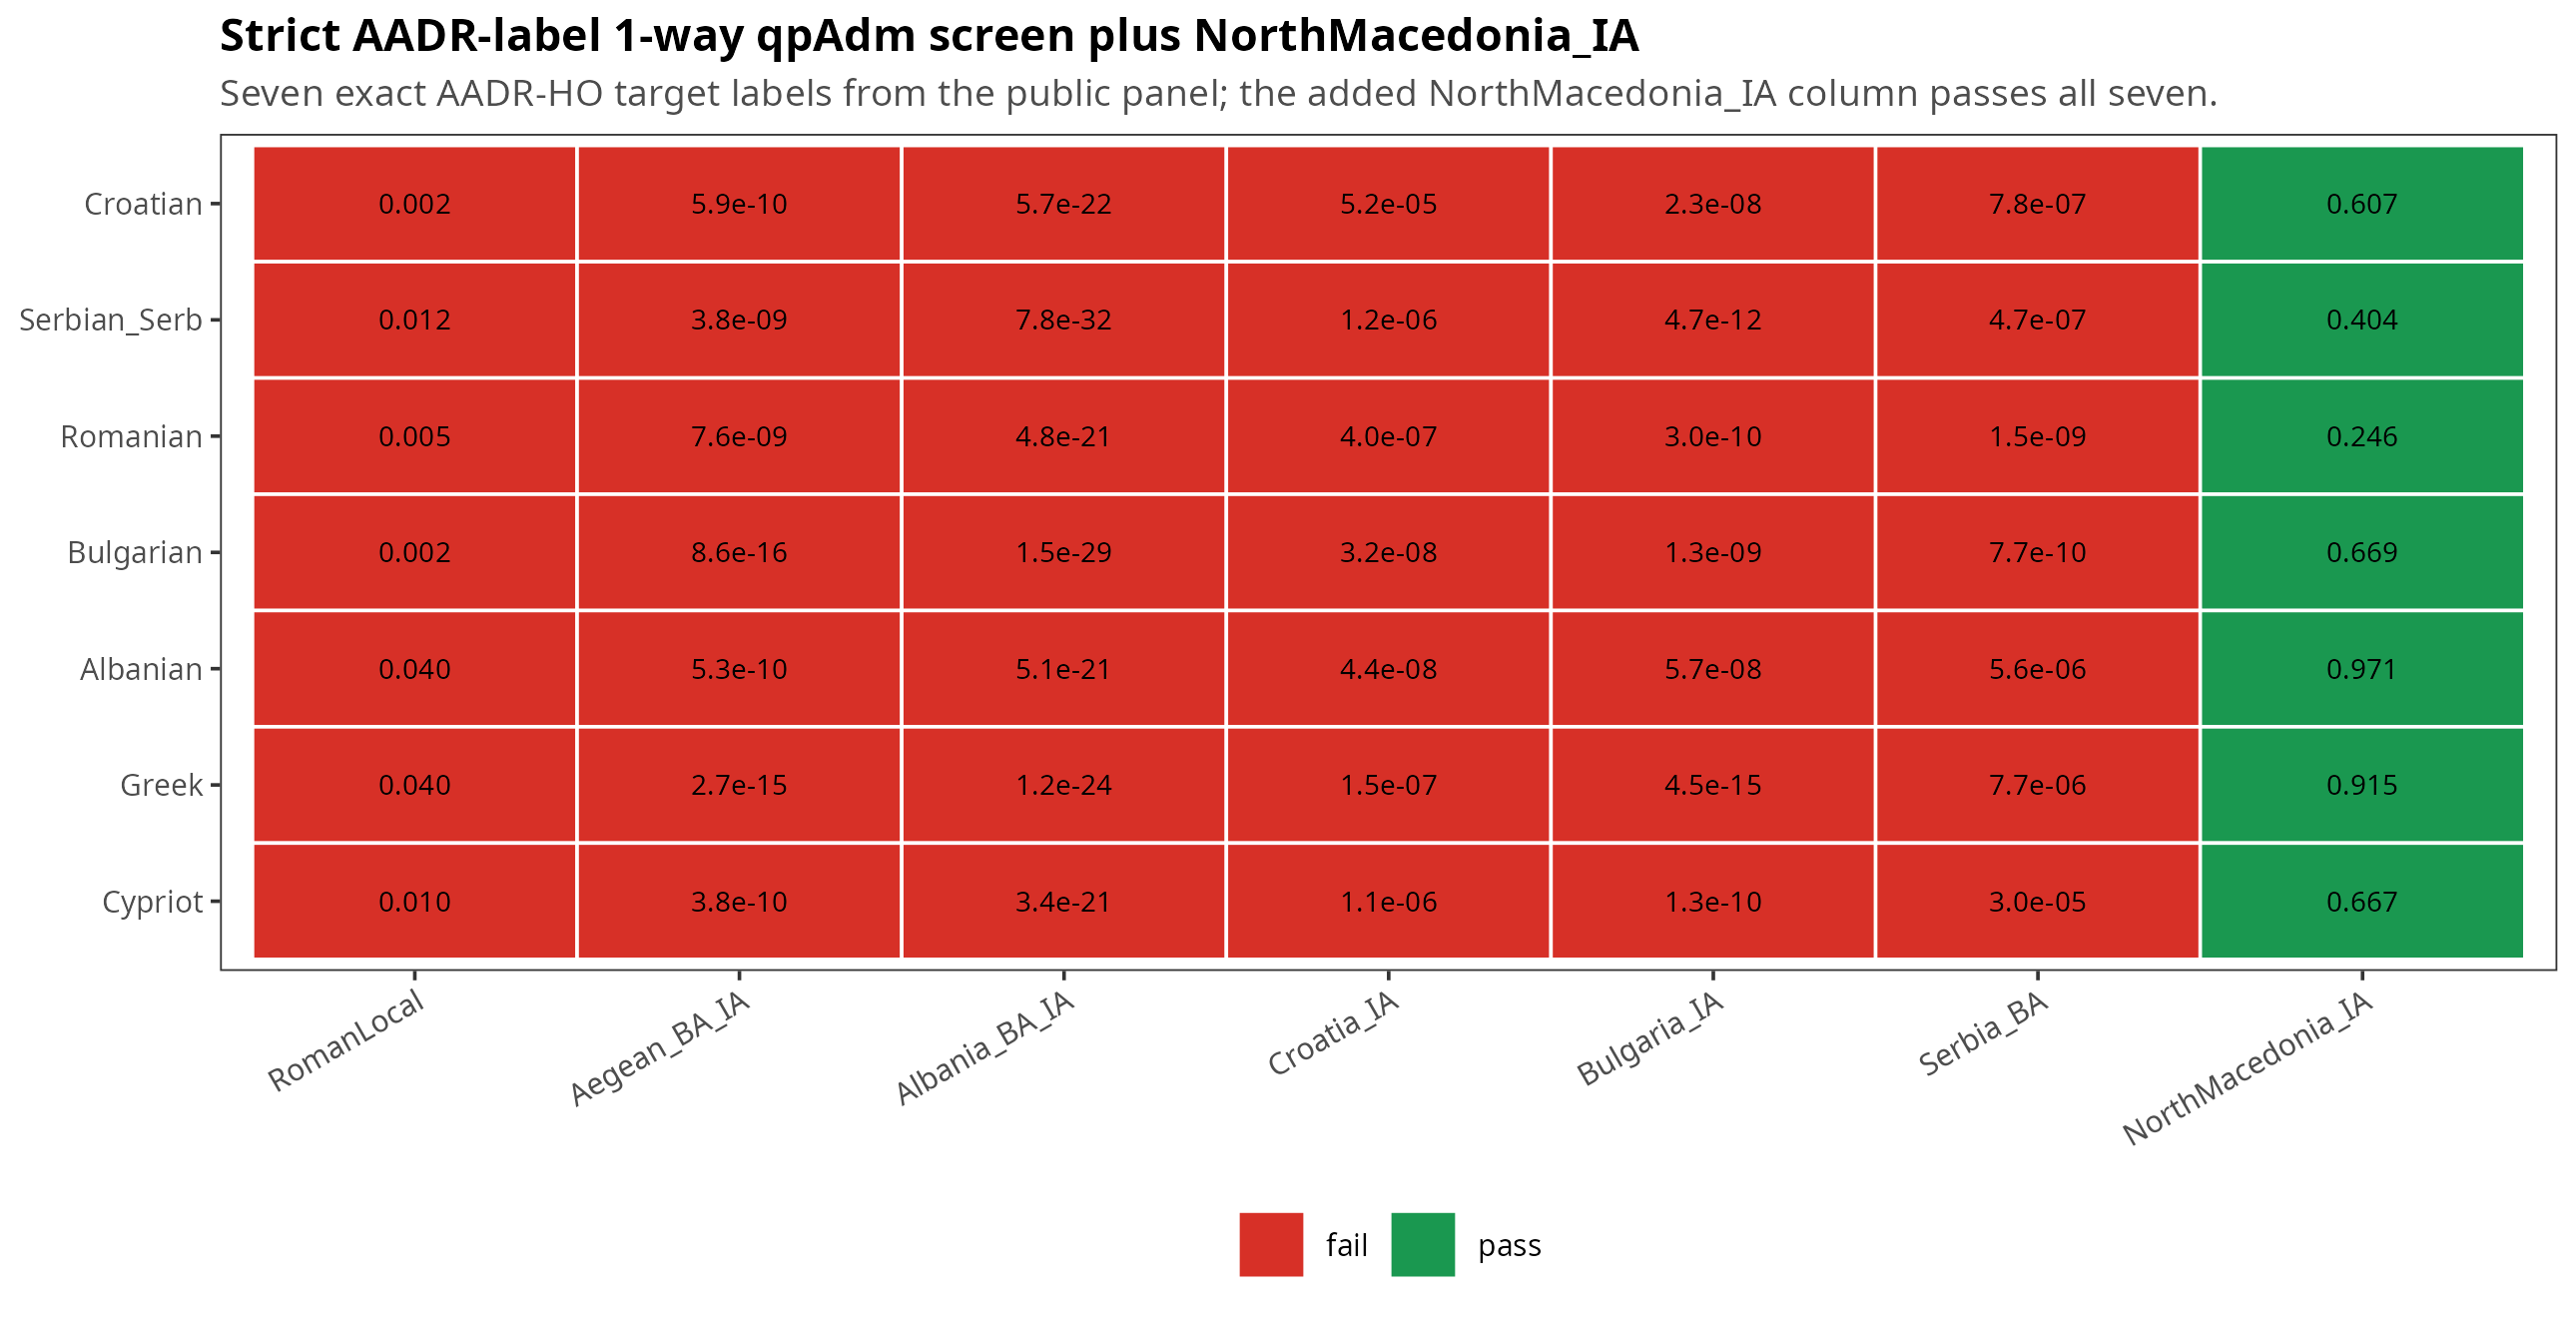
\includegraphics[width=\textwidth]{figs/fig1_table8_oneway.png}
  \caption{Strict AADR-label 1-source qpAdm screen plus
    \texttt{NorthMacedonia\_IA}. Cells report qpAdm $p$-values under
    \texttt{allsnps=TRUE}; green indicates non-rejection ($p > 0.05$).}
  \label{fig:oneway}
\end{figure}

\begin{table}[H]
\centering
\caption{Strict AADR-label 1-way screen versus the added \texttt{NorthMacedonia\_IA} column.}
\label{tab:main}
\small
\begin{tabular}{l l r r l}
\toprule
Target & Best published source & Best published $p$ & \texttt{NorthMacedonia\_IA} $p$ & Verdict \\
\midrule
Croatian & CroatiaSerbia\_RomanLocal & 0.002 & 0.607 & passes \\
Serbian\_Serb & CroatiaSerbia\_RomanLocal & 0.012 & 0.404 & passes \\
Romanian & CroatiaSerbia\_RomanLocal & 0.005 & 0.246 & passes \\
Bulgarian & CroatiaSerbia\_RomanLocal & 0.002 & 0.669 & passes \\
Albanian & CroatiaSerbia\_RomanLocal & 0.040 & 0.971 & passes \\
Greek & CroatiaSerbia\_RomanLocal & 0.040 & 0.915 & passes \\
Cypriot & CroatiaSerbia\_RomanLocal & 0.010 & 0.667 & passes \\
\bottomrule
\end{tabular}
\end{table}

\FloatBarrier

\section{Introduction}

\citet{Olalde2023} model Balkan population history with qpAdm using a fixed
right-set and a series of pre-Slavic Balkan substrates. For present-day
Balkan and Aegean groups, their workflow begins with a 1-source screen in
Data~S1 \S5 and Data~S2 Table~8, followed by target-specific multi-source
models. The reproducible step addressed here is that first-stage 1-source
screen.

This comment uses a strict public-label test rather than proxy relabeling of
every printed Table~8 row. The printed local 1-source rows include
\texttt{Croatian}, \texttt{Serbian}, \texttt{Romanian}, \texttt{Bulgarian},
\texttt{Albanian}, and several regional Greek labels listed in Supplementary
Table~S2. The analysis therefore stays with the exact public AADR Human
Origins labels available in the processed dataset: \texttt{Croatian},
\texttt{Serbian\_Serb}, \texttt{Romanian}, \texttt{Bulgarian},
\texttt{Albanian}, \texttt{Greek}, and \texttt{Cypriot}. The question is
simple: on this strict seven-label public panel, does adding the omitted Iron
Age Balkan cluster \texttt{NorthMacedonia\_IA} materially change the pass/fail
pattern?

That omitted cluster matters because it was available well before
\citet{Olalde2023}. The 14 \texttt{NorthMacedonia\_IA} individuals were
published in \citet{Lazaridis2022}, the same paper that supplied multiple
Iron Age Balkan substrates used by Olalde, and Iosif Lazaridis is a coauthor
of both studies. This is therefore not a case of importing a later or
peripheral candidate from outside the relevant literature, but of an obvious
candidate from the same immediate authorial and evidentiary context being left
out of the published stress test.

\section{Methods}

\subsection{Data and published setup}

\begin{sloppypar}
Genotypes are taken from the Allen Ancient DNA Resource v66.0 Human Origins
variant~\citep{AADRv66}. The present-day analysis considered here is the
published 1-source screen documented by \citet{Olalde2023} for Balkan and
Aegean populations. The documented right-set is:
\nolinkurl{OldAfrica}, \nolinkurl{Steppe_BA}, \nolinkurl{EHG},
\nolinkurl{Iron_Gates_HG}, \nolinkurl{Anatolia_N}, \nolinkurl{Iran_N},
\nolinkurl{Iberia_IA}, \nolinkurl{Greece_Minoan},
\nolinkurl{CroatiaMLBA_SloveniaIA}, \nolinkurl{Netherlands_MBA_IA},
\nolinkurl{Steppe_IA}, \nolinkurl{SoutheastTurkey_Byzantine}, and
\nolinkurl{Baltic_BA}.

The six published source columns are represented here by the public labels
\nolinkurl{CroatiaSerbia_RomanLocal}, \nolinkurl{Aegean_BA_IA},
\nolinkurl{Albania_BA_IA}, \nolinkurl{Croatia_IA},
\nolinkurl{Bulgaria_IA}, and \nolinkurl{Serbia_BA}; in Olalde's printed
Table~8, the corresponding Bulgaria column is labeled \nolinkurl{Bulgaria_EIA}.
We reproduce that screen under the same setup and then add
\nolinkurl{NorthMacedonia_IA} as a seventh, explicitly new column.

The retained target panel is the exact public-HO set used in the pipeline:
\texttt{Croatian}, \texttt{Serbian\_Serb}, \texttt{Romanian},
\texttt{Bulgarian}, \texttt{Albanian}, \texttt{Greek}, and
\texttt{Cypriot}. It is therefore a strict public-label panel, not a row-for-row
reproduction of every printed Table~8 target. Supplementary Table~S2 lists
these labels and the exclusion policy.
\end{sloppypar}

\subsection{Implementation}

\begin{sloppypar}
qpAdm models were computed in ADMIXTOOLS~2~\citep{Maier2023}. Olalde ran
classic ADMIXTOOLS with \nolinkurl{allsnps:YES}; in ADMIXTOOLS~2 the closest
match is \nolinkurl{qpadm(allsnps=TRUE)}, which reads from the genotype files
directly rather than from a global $f_2$ cache. The present analysis uses
that \nolinkurl{allsnps=TRUE} implementation for the published 1-source screen
and for the added \nolinkurl{NorthMacedonia_IA} column.

A 1-source qpAdm pass is treated here as non-rejection under this right-set and
dataset. It is not, by itself, a claim of literal historical ancestry or of
robustness to alternative right-sets and source rotations.
\end{sloppypar}

\section{Results}

\subsection{The reproduced 1-source screen still rejects every published substrate}

\begin{sloppypar}
Figure~\ref{fig:oneway} and Table~\ref{tab:main} summarize the strict
seven-label result. On the retained public-HO panel, every one of Olalde's six
published 1-source substrate columns still fails every row under
\nolinkurl{allsnps=TRUE}. The best published p-value in each row is achieved by
\nolinkurl{CroatiaSerbia_RomanLocal} and remains below the conventional
acceptance threshold, ranging from \BestPublishedMinP{} (\texttt{\BestPublishedMinTarget{}})
to \BestPublishedMaxP{} (\texttt{\BestPublishedMaxTarget{}}).
\end{sloppypar}

This reproduces the qualitative point of Olalde's own first-stage screen: none
of the published local substrates passes on this strict public-data subset
under the documented right-set.

\subsection{Adding \texttt{NorthMacedonia\_IA} changes the pass/fail pattern completely}

When \texttt{NorthMacedonia\_IA} is appended as a seventh source column under
the same setup, the pattern changes sharply. All seven retained target rows
pass, with p-values from \NorthmacMinP{} (\texttt{\NorthmacMinTarget{}}) to \NorthmacMaxP{}
(\texttt{\NorthmacMaxTarget{}}); see Table~\ref{tab:main}. This is a material change in
the first-stage screen, not a marginal numerical perturbation.

The implication is immediate. Even before any later model choice about Slavic,
Anatolian, or Roman-period components, this strict public-label test shows that
the published local substrate set was not exhaustive. An Iron Age Balkan
substrate absent from the published table is less strongly rejected than all
six published candidates and, in this implementation of Olalde's documented
setup, is not rejected at all on the retained panel.

\section{Discussion}

The point of this comment is narrow but consequential. In the strict
public-label restatement of the published present-day 1-source qpAdm screen,
all six of Olalde's published local substrate columns are rejected across the
retained target panel, whereas the omitted \texttt{NorthMacedonia\_IA} column
is not rejected in any retained row. That is enough to show that the published
screen was not exhaustive with respect to plausible Iron Age Balkan substrate
candidates.

Methodologically, that point is straightforward. In \citet{Olalde2023}, the
first-stage screen functions as a filter on later model choice. If a relevant
and previously available Iron Age Balkan candidate within the same broad
temporal and geographic frame was omitted, and adding it reverses the
pass/fail pattern of the screen, then the entry point of the model family
depends materially on source choice. The strict public-label panel does not
weaken that inference: on the exact public targets analyzed here, the
published six-source set fails uniformly while the omitted
\texttt{NorthMacedonia\_IA} source does not. This does not imply that
\texttt{NorthMacedonia\_IA} was a literal ancestor or that a 1-source qpAdm
pass establishes continuity. It does show that this source dependence should be
recognized explicitly.

\section*{Data and code availability}

All analysis code, intermediate results, and the LaTeX source are available at
\href{https://github.com/nikolatsartsarov/olalde2023_substrate_comment/}{the GitHub repository}.
Genotype data are not redistributed; researchers must download the AADR
v66.0 Human Origins dataset directly from the Harvard Dataverse release.

\bibliography{refs}

\end{document}
